\label{Dataset}
\subsection{Dataset}
En esta sección se detallan las especificaciones de los conjutnos de datos o datasets utilizados para entrenar el modelo YOLO.

\subsubsection{Pre-entrenamiento}
El modelo se entrenó desde cero (sus pesos establecidos aleatoriamente) usando el famoso dataset: VOC2012 Dataset \cite{voc2012}. Sus características principales son

\begin{itemize}
    \item Posee 20 clases. Figura \ref{fig:pascal-voc}
    \item Los datos de entrenamiento/validación contienen 11.530 imágenes comprendiendo 27.450 objetos anotados ROI (región de interés) y 6.929 objetos segmentados (no corresponde para object detection).
\end{itemize}

\begin{figure}[h!]
    \centering
    \begin{subfigure}[h]{\textwidth}
        \centering
        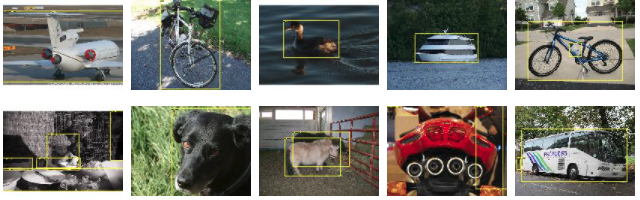
\includegraphics[width=\linewidth]{img/pascal-voc-20-classes-part1.png}
    \end{subfigure}
    \begin{subfigure}[h]{\textwidth}
        \centering
        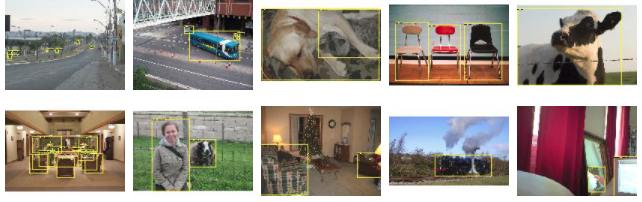
\includegraphics[width=\linewidth]{img/pascal-voc-20-classes-part2.png}
    \end{subfigure}
    \caption{Las 20 clases de VOC2012}
    \label{fig:pascal-voc}
\end{figure}

\newpage
\subsubsection{Formato de las Etiquetas} 
Un dataset se compone típicamente de un conjunto de imágenes y un conjunto de etiquetas asociadas a cada una de ellas. Dichas etiquetas respetan un formato estricto, que para el caso del presente proyecto es: ``Pascal Visual Object Classes (VOC)'', el cual está caracterizado por:

\begin{itemize}
    \item Es un archivo XML. Ejemplo de formato VOC2012 \cite{etiqueta} :
    
        \lstset{frame=tb,
            language=XML,
            morekeywords={encoding,
                annotation,folder,filename,path,source,
                database,size,width,heigth,depth,
                segmented,object,name,pose,truncated,
                difficult,bndbox,xmin,ymin,xmax,ymax
            }
        }
        \begin{lstlisting}
        <annotation>
            <folder>Kangaroo</folder>
            <filename>00001.jpg</filename>
            <path>./Kangaroo/stock-12.jpg</path>
            <source>
                <database>Kangaroo</database>
            </source>
            <size>
                <width>450</width>
                <heigth>319</heigth>
                <depth>3</depth>
            </size>
            <segmented>0</segmented>
            <object>
                <name>kangaroo</name>
                <pose>Unspecified</pose>
                <truncated>0</truncated>
                <difficult>0</difficult>
                <bndbox>
                    <xmin>233</xmin>
                    <ymin>89</ymin>
                    <xmax>386</xmax>
                    <ymax>262</ymax>
                </bndbox>
            </object>
        </annotation>
        \end{lstlisting}
    \item Se crea un archivo para cada imagen del dataset.
    \item Las etiquetas están definidas como: \[(\textit{xmin-top left, ymin-top left, xmax-bottom right, ymax-bottom right})\]
\end{itemize}

\newpage
\subsubsection{Dataset Personalizado}
El dataset con el cual se realizo el re-entrenamiento del modelo, esta basado en imágenes con vista satelital de pivotes y silobolsas extraídas de diferentes fuentes de acceso libre:
\begin{itemize}
    \item Usando la herramienta QGIS \cite{qgis} se obtuvieron imágenes satelitales de las fuentes: Sentinel, Google y Bing Sattelite.
    \item Google Maps
    \item Las etiquetas esta definidas como: \textit{(xmin-top left, ymin-top left,xmax-bottom right, ymax-bottom right)}
\end{itemize}

Las mismas poseen 3 bandas del espectro visible (RGB) y varían en tamaño, color, relación de aspecto de acuerdo a las diferentes estaciones del año y resolución, es decir, que tan cerca o lejos del nivel del mar se obtuvieron las imágenes. Se seleccionaron de tal manera que su distribución fuera uniforme: tantos objetos en solitario, como en conjunto, así como también balanceado, es decir, cada clase de objetos contenga la relativamente la misma cantidad.\\ 

La literatura y la práctica recomiendan un dataset “grande” para obtener resultados aceptables, lo que implica, como regla general:
\begin{itemize}
    \item Al menos 1500 imágenes por clase.
    \item Al menos 10000 instancias (objetos etiquetados) por clase.
\end{itemize}

Sin embargo ante la dificultad de seleccionar a mano un número tan grande de imágenes se optó por aplicar técnicas de Data Augmentation o Aumento de Datos, y de esta manera nos permite aumentar nuestro set de datos de entrenamiento para mejorar la precisión, la generalización, y controlar el overfitting:
\begin{itemize}
    \item Generación de Imágenes Sintéticas: Utilizando imágenes con diferentes colores y texturas como ``fondos'' e imágenes de los objetos de interés, se generaron nuevas imágenes sintéticas.
    \item Rotaciones: Se aplicaron rotaciones sobre las imágenes originales y las sintéticas
\end{itemize}

Finalmente el dataset quedó compuesto por decenas de miles de imágenes, algunas etiquetadas manualmente y en su gran mayoría imágenes similares a las que se muestran en el Anexo \ref{anexo:dataset}:

\newpage
\paragraph{Distribución de Etiquetas}
\begin{figure}[h!]
    \centering
    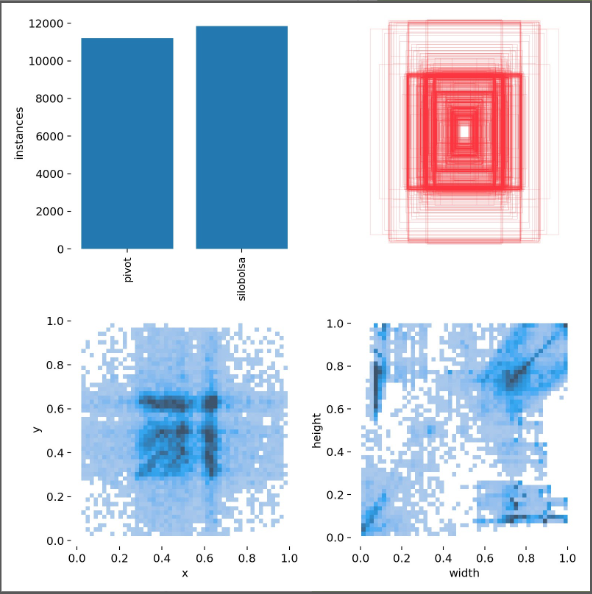
\includegraphics[width=0.95\textwidth]{img/distribucion de etiquetas.png}
    \caption{Distribución de Etiquetas}
    \label{fig:distribucion de etiquetas}
\end{figure}

De la anterior Figura \ref{fig:distribucion de etiquetas} se observan las siguientes conclusiones:
\begin{itemize}
    \item En el gráfico de barras ubicado en la esquina superior izquierda de la figura, se puede ver la distribución de etiquetas por clase. Notar que están relativamente balanceadas: con casi la misma cantidad de pivotes que de silobolsas.
    \item En la imagen superior derecha , se ven en rojo los diferentes bounding box (BB) que suelen ser en su mayoría cuadrados perfectos (pivotes y silobolsas en diagonal) de gran tamaño o bien muy pequeños, por lo que se concentran en la esquina superior derecha (1,1) e inferior izquierda (0,0).
    \item También se denota una gran concentración de BB altos y angostos  en la esquina superior izquierda (0,1) y anchos y bajos en la esquina inferior derecha (1,0), los cuales se corresponden a etiquetas de silobolsas de grandes dimensiones ubicadas vertical y horizontalmente respectivamente.
    \item En el gráfico ubicado en la esquina inferior izquierda se observa que el centro de los BB suele concentrarse en el centro de las imágenes y sobre todo evitan las esquinas.
\end{itemize}

\paragraph{Correlograma de Etiquetas}
\begin{figure}[h!]
    \centering
    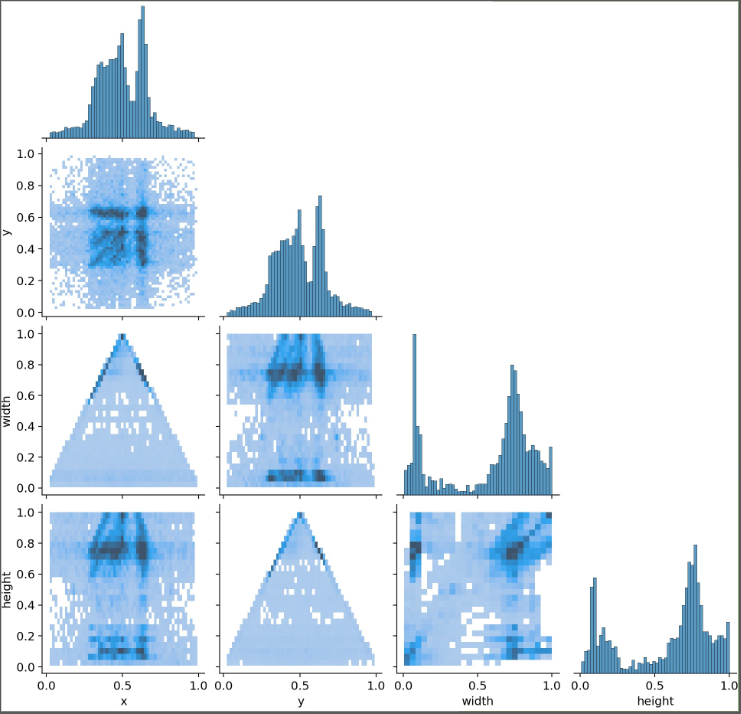
\includegraphics[width=1\textwidth]{img/correlograma de etiquetas.png}
    \caption{Correlograma de Etiquetas: nos ayudan a visualizar la correlación entre las etiquetas de los objetos. }
    \label{fig:correlograma de etiquetas}
\end{figure}

De la anterior Figura \ref{fig:correlograma de etiquetas} se observan las siguientes conclusiones:
\begin{itemize}
    \item La distribución de los BB se concentran en el centro de las imágenes, y sobre todo evitan las esquinas (x,y). 
    \item La distribución del ancho y alto de los BB denota que son cuadrados, o bien, rectángulos alargados tanto horizontales como verticales (width,height).
    \item Los BB ubicados en el centro del eje X de las imágenes tienden a ser extremadamente altas o bajas (x,height).
    \item Los BB ubicados en el centro del eje Y de las imágenes tienden a ser extremadamente anchas o angostas (y,width).
\end{itemize}
